%% 
%% Copyright 2007, 2008, 2009 Elsevier Ltd
%% 
%% This file is part of the 'Elsarticle Bundle'.
%% ---------------------------------------------
%% 
%% It may be distributed under the conditions of the LaTeX Project Public
%% License, either version 1.2 of this license or (at your option) any
%% later version.  The latest version of this license is in
%%    http://www.latex-project.org/lppl.txt
%% and version 1.2 or later is part of all distributions of LaTeX
%% version 1999/12/01 or later.
%% 
%% The list of all files belonging to the 'Elsarticle Bundle' is
%% given in the file `manifest.txt'.
%% 

%% Template article for Elsevier's document class `elsarticle'
%% with numbered style bibliographic references
%% SP 2008/03/01

\documentclass[preprint,12pt, a4paper]{elsarticle}

%% Use the option review to obtain double line spacing
%% \documentclass[authoryear,preprint,review,12pt]{elsarticle}

%% For including figures, graphicx.sty has been loaded in
%% elsarticle.cls. If you prefer to use the old commands
%% please give \usepackage{epsfig}

%% The amssymb package provides various useful mathematical symbols
\usepackage{amssymb}
%% The amsthm package provides extended theorem environments
%% \usepackage{amsthm}

%% The lineno packages adds line numbers. Start line numbering with
%% \begin{linenumbers}, end it with \end{linenumbers}. Or switch it on
%% for the whole article with \linenumbers.
\usepackage{lineno}
\usepackage{hyperref}
\usepackage{listings}
\usepackage{pdflscape}

\lstset{ 
  language=R,                      % the language of the code
  basicstyle=\scriptsize\ttfamily, % the size of the fonts that are used for the code
  backgroundcolor=\color{white},   % choose the background color. You must add \usepackage{color}
  showspaces=false,                % show spaces adding particular underscores
  showstringspaces=false,          % underline spaces within strings
  showtabs=false,                  % show tabs within strings adding particular underscores
  frame=single,                    % adds a frame around the code
  rulecolor=\color{black},         % if not set, the frame-color may be changed on line-breaks within not-black text (e.g. commens (green here))
  tabsize=2,                       % sets default tabsize to 2 spaces
  captionpos=b,                    % sets the caption-position to bottom
  breaklines=true,                 % sets automatic line breaking
  breakatwhitespace=false,         % sets if automatic breaks should only happen at whitespace
  keywordstyle=\color{RoyalBlue},   % keyword style
  commentstyle=\color{PineGreen},   % comment style
  stringstyle=\color{RubineRed}     % string literal style
} 


\usepackage[usenames,dvipsnames]{color}    

\usepackage{float}
\restylefloat{table}

\journal{SoftwareX}

\begin{document}

\begin{frontmatter}

%% Title, authors and addresses

%% use the tnoteref command within \title for footnotes;
%% use the tnotetext command for theassociated footnote;
%% use the fnref command within \author or \address for footnotes;
%% use the fntext command for theassociated footnote;
%% use the corref command within \author for corresponding author footnotes;
%% use the cortext command for theassociated footnote;
%% use the ead command for the email address,
%% and the form \ead[url] for the home page:
%% \title{Title\tnoteref{label1}}
%% \tnotetext[label1]{}
%% \author{Name\corref{cor1}\fnref{label2}}
%% \ead{email address}
%% \ead[url]{home page}
%% \fntext[label2]{}
%% \cortext[cor1]{}
%% \address{Address\fnref{label3}}
%% \fntext[label3]{}

\title{pksensi: an R Package to Apply Global Sensitivity Analysis in
Physiologically Based Kinetic Modeling}

%% use optional labels to link authors explicitly to addresses:
%% \author[label1,label2]{}
%% \address[label1]{}
%% \address[label2]{}

\author[1]{Nan-Hung Hsieh}
\author[2]{Brad Reisfeld}
\author[1]{Weihsueh A. Chiu\corref{cor}}
\ead{wchiu@cvm.tamu.edu}
\cortext[cor]{Corresponding author}

\address[1]{
Veterinary Integrative Biosciences, College of Veterinary Medicine and
Biomedical Sciences, Texas A\&M University, College Station, TX, USA\\
}
\address[2]{
Chemical and Biological Engineering and School of Biomedical
Engineering, Colorado State University, Fort Collins, CO, USA\\
}


\begin{abstract}
%% Text of abstract 
Sensitivity analysis (SA) is an essential tool for modelers to understand the influence of model parameters on model outputs. It is also increasingly used in developing and assessing physiologically based kinetic (PBK). For instance, we applied a global SA workflow to reduce the computational burden in the Bayesian Markov Chain Monte Carlo-based calibration process of a physiologically based pharmacokinetic model. Although several SA algorithms and software packages are available, no comprehensive software package exists that allows users to seamlessly solve differential equations in the PBK model, conduct and visualize SA results, and discriminate between the non-influential model parameters that can be fixed and those that need calibration.  Therefore, we developed an R package, named \textbf{pksensi}, to make global SA more accessible in PBK modeling. This package can investigate both uncertainty and sensitivity in PBK models, including those with multivariate model outputs. It also includes functions to check the convergence of the global SA results. Overall, \textbf{pksensi} improves the user experience of performing global SA and can create robust and reproducible results for decision making in PBK model calibration.

\end{abstract}

\begin{keyword}
  Global sensitivity analysis \sep Physiologically based kinetic modeling \sep R package

%% PACS codes here, in the form: \PACS code \sep code

%% MSC codes here, in the form: \MSC code \sep code
%% or \MSC[2008] code \sep code (2000 is the default)

\end{keyword}

\end{frontmatter}

\newpage

\section*{Required Metadata}

\section*{Current code version}

\begin{table}[H]
\begin{tabular}{|l|p{6.5cm}|p{6.5cm}|}
\hline
\textbf{Nr.} & \textbf{Code metadata description} & \textbf{Please fill in this column} \\
\hline
C1 & Current code version & 1.2.0 \\
\hline
C2 & Permanent link to code/repository used for this code version & \url{https://github.com/nanhung/pksensi} \\
\hline
C4 & Legal Code License & LPGL-3.0 \\
\hline
C5 & Code versioning system used & git \\
\hline
C6 & Software code languages, tools, and services used & R \\
\hline
C7 & Compilation requirements, operating environments \& dependencies & ggplot2, data.table, deSolve, dplyr, getPass, magrittr, foreach, parallel, doParallel, reshape \\
\hline
C8 & If available Link to developer documentation/manual & \url{https://nanhung.rbind.io/pksensi/} \\
\hline
C9 & Support email for questions & \url{d99622005@ntu.edu.tw} \\
\hline
\end{tabular}
\caption{Code metadata (mandatory)}
\label{} 
\end{table}


\linenumbers

%% main text

\newpage

\section{Motivation and significance}

Sensitivity analysis (SA) is a mathematical technique to investigate how variations in model parameters affect model outputs. An increasing number of studies use SA to determine which model parameters contribute to high variation in model predictions \cite{ferretti2016trends}. This technique has also been applied in pharmacology and toxicology research \cite{loizou2015application, mcnally2012reconstruction}. Pharmacokinetic models describe the changes in the concentrations or amounts of a substance in the body over time (the various terms for the kinetic models, including ``pharmacokinetic'', ``toxicokinetic'', and ``biokinetic'' models, are used exchangeably here). The goal of SA in physiologically based kinetic (PBK) research is to examine the sensitivity of output variables, such as chemical concentration in blood or tissues, with respect to input parameters, such as anatomical, physiological, and kinetic constants \cite{mcnally2011workflow}. In addition, this SA approach can guide experimental design and the parameter estimation processes \cite{zhang2015sobol}. For instance, SA can identify ``unidentifiable'' parameters that can lead to problems with numerical procedures used in parameter estimation \cite{chu2010quantitative}. It can be further applied to parameter prioritization and parameter fixing before model calibration \cite{fphar201800588}.

In our earlier work \cite{fphar201800588}, we developed an updated workflow to apply global SA to reduce the computational burden in the Bayesian, Markov Chain Monte Carlo (MCMC)-based calibration process of a physiologically based pharmacokinetic (PBPK) model. We used GNU MCSim \cite{bois2009gnu}, an effective simulation package for Bayesian population PBPK modeling, to calibrate the model. We found that the extended Fourier Amplitude Sensitivity Test (eFAST), a type of variance-based global SA algorithm, had the best balance of efficiency and accuracy for a sophisticated, multi-compartment, multi-dataset, and multi-metabolite PBPK model. This method was first introduced in 1973,  \cite{cukier1973study} in a study of the sensitivity of coupled reaction systems that are constructed by differential equations with the numerous rate coefficients (the classic FAST method with the first-order effect only). It then evolved to estimate the Sobol' sensitivity measure (the eFAST method with first- and total-order effects) \cite{saltelli1999quantitative}. The FAST algorithm creates the multidimensional space of input parameters through a ``search-curve''. It is more computationally efficient in calculating the influence of model parameters than other global SA methods such as the Monte Carlo based approaches \cite{jansen1999analysis, owen2013better}. Our previous work also found some efficient visualization approaches that can be used to distinguish between ``influential'' and ``non-influential'' parameters. This approach addresses common identifiability issues of PBPK model parameter that increase the computational burden of Bayesian analysis \cite{garcia2015identifiability}, and therefore reduce the computational efficiency. We also developed approaches for communicating parameter sensitivity in decision making.

Most of SA tools are constructed using scientific computing software, 
such as Matlab \cite{pianosi2015matlab}, python \cite{herman2017salib}, and R \cite{iooss2017introduction}. The R software is widely used and includes numerous developed packages, such as \textbf{sensitivity} \cite{R-sensitivity}, which is a practical tool to conduct local and global SA. The \textbf{sensitivity} package includes some functions to generate the parameter sequences by using different computing algorithms. Also, it provides a feasible way to integrate external modeling results. This computational approach can effectively solve the heavy computing burden of numerical solutions within the pure R environment. 

Several other R packages include SA tools and are freely available in the Comprehensive R Archive Network (CRAN). Although these tools provide various approaches to perform SA, they each individually have limitations for application to PBK modeling. For example, the estimated index in SA is not robust when using the inadequate size of the sample number. However, there are no software packages that provide the available tools in the assessment of reliability. In addition, the existing eFAST function does not include the feature to generate the random sampling curve. We present here an R package, called \textbf{pksensi}, which is designed to make SA more accessible and reproducible in pharmacological and toxicological researches. 


\section{Software description}

Our package can investigate both parameter uncertainty and sensitivity in PBK model with multivariate model outputs. Moreover, it seamlessly integrates with both general ODE solvers available in R or as external C code, as well as the GNU MCSim software used for conducting sophisticated PBK modeling, including MCMC. The analytical framework in \textbf{pksensi} includes not only global SA but also the uncertainty analysis and diagnostic tools to support the modeling process.


\subsection{Installation}

This package can link with R \textbf{deSolve} package, which includes a comprehensive integrator to solve ODE. The GNU MCSim can be installed by following the instruction in GNU MCSim's manual on \url{https://www.gnu.org/software/mcsim/mcsim.html} or using the built-in function in \textbf{pksensi}.

\subsection{Parameter matrix generation}

We adopted eFAST, the widely used analysis of variance (ANOVA)-like global SA approach to decompose the variance to partial variances for multidimensional parameters in numerical models in this package. Most of the available eFAST functions, such as the algorithm to generate the parameter space and to set the sampling frequency, were sourced from the R \textbf{sensitivity} package \cite{R-sensitivity}. The eFAST method computes the sensitivity index (SI) via ANOVA-like decomposition of the function for analysis. This type of global SA approach and SI also know as Sobol' method and Sobol' index. Since the estimated SI is not stable (high variation) when using smaller sample size, we included a random phase-shift approach to conduct replicating sampling from random starting points across parameter space to test the convergence and robustness of the sensitivity measurement. Considering the model that is built under \(y=f(x_{i})\). The sampling scheme can describe as,

\[ x_i = \frac{1}{2} + \frac{1}{\pi}\arcsin(\sin(\omega_is + \varphi_i)) \]

where \(x_i\) is the nominal value of the \(i\)-th parameter, and \(\omega_i\) is a vector giving the set of frequencies, one frequency for each parameter, and \(\varphi\) is a random phase-shift coefficient
ranged from 0 to \(2\pi\). Through the random phase-shift, the robust result of the sensitivity measurement should be similar across each replication under the same sample size. For most Sobol'-based SA algorithms, the larger sample size is needed to reduce the probability of having negative estimates. However, eFAST estimates are always positive according to its construction.

To investigate the convergence of SI, we adopted the ``exam'' approach that proposed previously \cite{sarrazin2016global}. This method quantitatively assesses convergence by computing the width of 95\% confidence intervals of computed SI for all parameters across all time-points and output variables. Through the random phase-shift procedure, the replicated SI values can repeatedly sample independently. Therefore, they can be used to investigate the convergence of SI as,

\[CI_{i,t} = max(SI_{i,t}^{ub}-SI_{i,t}^{lb})\]

where \(SI_{i,t}^{ub}\) and \(SI_{i,t}^{ub}\) are the upper and lower bound of the SI from the specific model output (\(i\)) at time (\(t\)). \(CI_{i,t}\) is the corresponding convergence index.

\textbf{pksensi}, we integrate the random phase-shift with eFAST to perform the sensitivity test for the whole modeling process. The function can sample and generate the testing parameter matrix based on a given argument of sample size and probability distribution (e.g., mean/s.d. of normal distribution, meanlog/sdlog of log-normal distribution, and minimum/maximum of uniform distribution). The number of model evaluations is equal to the sample size times the number of model parameters.


\subsection{Modeling}

The \textbf{pksensi} provides a useful function to solve ODEs in PBK models using analytical and numerical approaches. The solution can perform under the pure R programming environment by linking with R deSolve package \cite{JSSv033i09}. However, the most efficient way to achieve high computational speed is through compiled, lower-level languages, such as FORTRAN, C, or C++. Therefore, it includes a function to compile and create dynamic-link libraries (.dll) on Windows and shared objects (.so) on Unix-liked systems (e.g., Linux and MacOS). This compiled program can load and execute through the build-in function in R. However, Windows users need to install Rtools to compile the source code by using the GNU GCC compiler. The C implementation of the example model can be found as an example within GNU MCSim \cite{bois2009gnu}. The \textbf{pksensi} can also link with GNU MCSim to create the model program, used in solving each system of equations. 


\subsection{Uncertainty analysis}

\textcolor{red}{The general workflow of uncertainty and SA in \textbf{pksensi} is illustrated in Figure \ref{fig:workflow}. The uncertainty analysis is a crucial modeling process within SA. Sometimes, it is difficult to have informative data to set up the parameter distribution. A wider range for a parameter distribution might cause a numerical error at extreme values. On the other hand, narrower ranges might cause the incorrect calibrated result of the model parameter. The uncertainty analysis using Monte Carlo is an appropriate approach in the data-driven modeling process to address this problem. Before fitting the data to model, the Monte Carlo can be applied with the given distribution of model parameters to examine whether the experimental data are within the ``rational" range of the distribution of model output. The \textbf{pksensi} also has a function that can link to GNU MCSim to conduct Monte Carlo analysis, which is built-into GNU MCSim and examine the simulation result. In addition, the users can also examine the model output that was generated by the parameter matrix from eFAST.}


\subsection{Sensitivity analysis}

\textcolor{red}{Through the plotting functions in \textbf{pksensi}, time-dependent sensitivity measurements of first and total effects for all parameters can be plotted simultaneously. If the computed sensitivity indices show different values across replications under the same sample size, this indicates an inadequate sample number, which can create an unreliable result. It is essential to use a sufficient sample size to prevent incorrect judgments in parameter fixing. The package includes functions to check the convergence and sensitivity of model parameters, providing a means to assess the robustness of the sensitivity measurement. We also developed a ``cut-off''-based approach in this package to distinguish between ``influential'' and ``non-influential'' parameters. Finally, this package also provides visualization tools for effective investigation and communication of results in decision support.}


\section{Illustrative Examples}

We currently proposed two example models to illustrate using \textbf{pksensi} in PBK modeling. In the first example, we used a generic, one-compartment model from \textbf{httk} package \cite{JSSv079i04} to explain the overall workflow and the details in the simulation process. Users can refer to online vignettes and user manual in the CRAN (\url{https://cran.r-project.org/web/packages/pksensi/index.html}) or the \textbf{pksensi} website (\url{https://nanhung.rbind.io/pksensi/}) for the detailed usage examples. The partial example of the R code and its result is given in Appendix A and Figure \ref{fig:example-1} that comprises the following essential steps in the process.

\begin{enumerate}
  \item Construct the model
  \item Define initial conditions, output time steps and variables
  \item Set parameter distributions
  \item \textcolor{red}{Conduct simulation}
  \item \textcolor{red}{Uncertainty analysis}
  \item \textcolor{red}{Check and visualize SA result}
\end{enumerate}

The first step is to prepare and construct the model. The model code can be written based on R \textbf{deSolve} and GNU MCSim format to provide the flexibility for the user. Then, setting up the variables and its initial conditions for the prepared model. Also, the simulation time points have to provided in this part.

\textcolor{red}{The third step is to identify the model parameters that will be examed in global SA and create the parameter matrix. After the parameter selection, we have to assign the corresponding value in probability function, such as minimum and maximum in a uniform distribution. After the definition, the users can use \textit{\textbf{rfast99()}} with the assignments (e.g., parameter names, sample number, parameter distribution, and its corresponding properties) that were defined in the above steps to create parameter matrix.}

Finally, solve the ODE in the model by using the \textit{\textbf{solve\_fun()}} function and visualize the result. The result of the one-compartment model shows that body weight (BW) is a non-influential parameter for the blood concentration in the simulation (see Appendix). In addition, use model code and solving engine from GNU MCSim (\textit{\textbf{solve\_mcsim()}}) can provide the fastest computational speed.

The second example used acetaminophen (APAP)-PBPK model, 
a complex model with multiple compartments, to demonstrate the reproducibility of our previous publication \cite{fphar201800588} and the capability of \textbf{pksensi}. The APAP-PBPK model describes the pharmacokinetics of parent APAP and its two metabolites glucuronide \(AG\) and sulfate \(AS\). We applied the comprehensive global SA workflow to the original published model with 21 model parameters \cite{s13318-015-0253-x}. Figure \ref{fig:example-2} shows the time-dependent total SI computed for the global SA method. The heat map provides an alternative way to visualize the estimated results. Some parameters (e.g., \(CYP\_Km\)) showed the non-influential impact across all three output variables across the investigation time interval.


\section{Impact and conclusions}

Computational modeling has become an essential technique in modern scientific research to support hypotheses, experiments, and discoveries. Uncertainty and SA are essential tools for modelers in the conduct of model development and examination. Several packages on the CRAN repository and other software platforms had been built to perform global SA with a variety of algorithms, but none have included integration with ODE-based models, such as PBK models. 

We initiated \textbf{pksensi} in order to facilitate a comprehensive and efficient global SA workflow in PBK modeling, filling a crucial gap for open-source modeling communities. It provides a straightforward
application to investigate the impact of parameters on model outputs across simulation time-points and variables. We adopted the eFAST method, a common variance-based SA that we found to have the best
balance of efficiency and accuracy. In addition, the package also includes the ability to assess the convergence of SA results, which is rarely addressed in most global SA studies and software packages. We also developed functions to visualize the output results and help distinguish the ``influential'' and ``non-influential'' parameters that can be applied in parameter fixing in the model calibration. Our package make global sensitivity analysis more accessible in PBK modeling.

We chose to integrate sensitivity analysis with GNU MCSim because it is a powerful open-source software package for dynamical simulation of biological-based models, mainly built for PBK research with probabilistic approaches \cite{bois2009gnu}. In addition, the current version of \textbf{pksensi} includes both GNU MCSim and \textbf{deSolve} package as the main ODE solvers. Compared with the \textbf{deSolve} package, the GNU MCSim can provide better speed and efficiency to solve the ODEs in PBK models. Although \textbf{pksensi} provides the essential features and functions to install and link with GNU MCSim, conducting the uncertainty and SA in PBK modeling, the overall learning curve of this workflow might steep for users that are not familiar with GNU MCSim from model development, debugging, and testing. Therefore, the general package, such as \textbf{deSolve}, can be an alternative option for R users. The flexibility of our package can help modelers quantify the influence of model parameters on model outputs. It addition, \textbf{pksensi} also has the potential to be performed in an interactive PBPK modeling platform that was mentioned in the recent study \cite{li2019integration}.

It is worth noting that the current global SA results are conditional on the specific model and the given range of the model parameters. Other factors, such as the number of parameters examined, the parameter distributions/ranges, and the given dosing level in the PBK model might also have a potential impact on the level of importance of each parameter, but these "meta-uncertainties" are not currently addressed. Complex models with high parameter dimensionality are also challenging in global SA as they have higher computer demands. As approaches are developed to address these complexities, we hope to incorporate them into \textbf{pksensi}.

Overall, \textbf{pksensi} provides a comprehensive suite of features and functions for performing global SA for PBK models and can create robust and reproducible results for decision making in model development and calibration. Although \textbf{pksensi} used here is mainly for PBK modeling, it can also be applied to other ODE-based dynamic models in order to investigate the sensitivity of model outputs to input parameters.

\section*{Conflict of Interest}

The authors declare that they have no known competing financial interests or personal relationships that could have appeared to influence the work reported in this paper.

\section*{Acknowledgements}

This work was funded, in part, by grant 1U01FD005838 from the U.S. Food and Drug Administration (FDA) and grant P42 ES027704 from the U.S. National Institute of Environmental Health Sciences. This article reflects the views of the author and should not be construed to represent FDA's views or policies. We thank Dr.~Yasha Hartberg and Dr.~Barbara Gastel at the Texas A\&M University, Dr.~Frederic Bois from Certara, and Dr.~Eleftheria Tsakalozou from U.S. FDA for reviewing the manuscript and consultation.

%% The Appendices part is started with the command \appendix;
%% appendix sections are then done as normal sections

\appendix
\section*{Appendix A. Example code}

\begin{lstlisting}
library(pksensi)
library(httk)

# Example: One-compartment pbtk model ------------------------------------
# Step 1. Construct 1-cpt pbtk model for deSolve package
pbtk1cpt <- function(t, state, parameters) {
  with(as.list(c(state, parameters)), {
    dAgutlument = - kgutabs * Agutlument
    dAcompartment = kgutabs * Agutlument - ke * Acompartment
    dAmetabolized = ke * Acompartment
    Ccompartment = Acompartment / vdist * BW;
    list(c(dAgutlument, dAcompartment, dAmetabolized), 
         "Ccompartment" = Ccompartment) 
  })
}

# Step 2. Define initial conditions, output time steps and variable
initState <- c(Agutlument = 10, Acompartment = 0, Ametabolized = 0)
t <- seq(from = 0.01, to = 24.01, by = 1)
outputs <- c("Ccompartment")

# Step 3. Generate parameter matrix 
## 3.1. Extract parameter value from httk package
pars1comp <- (parameterize_1comp(chem.name = "acetaminophen"))

## 3.2. Set parameter distributions
q <- c("qunif", "qunif", "qunif", "qnorm")
q.arg <- list(list(min = pars1comp$Vdist / 2, max = pars1comp$Vdist * 2),
              list(min = pars1comp$kelim / 2, max = pars1comp$kelim * 2),
              list(min = pars1comp$kgutabs / 2, max = pars1comp$kgutabs * 2),
              list(mean = pars1comp$BW, sd = 5))

## 3.3. Create parameter matrix
set.seed(1234)
params <- c("vdist", "ke", "kgutabs", "BW")
x <- rfast99(params, n = 200, q = q, q.arg = q.arg, replicate = 10)

# Step 4. Conduct simulation (will take few minutes)
out <- solve_fun(x, time = t, func = pbtk1cpt, initState = initState, outnames = outputs)

# Step 5. Uncertainty analysis
pksim(out)  # Use to compare with "real" data (if any)

# Step 6. Check and visualize the result of sensitivity analysis
plot(out)   # Visualize result
check(out)  # Print result to console
\end{lstlisting}

\section*{CRediT authorship contribution statement}

\textbf{Nan-Hung Hsieh:} Conceptualization, Software, Writing - Original Draft.
\textbf{Brad Reisfeld:} Funding acquisition, Project administration. 
\textbf{Weihsueh A. Chiu:} Supervision, Methodology, Writing - Review \& Editing. 

%% References:
%% If you have bibdatabase file and want bibtex to generate the
%% bibitems, please use
%%
%%  \bibliographystyle{elsarticle-num} 
%%  \bibliography{<your bibdatabase>}

%% else use the following coding to input the bibitems directly in the
%% TeX file.

\bibliographystyle{elsarticle-num} 
\bibliography{j.softx.pksensi}

\newpage

\clearpage
\newpage

\begin{landscape}

\begin{figure}
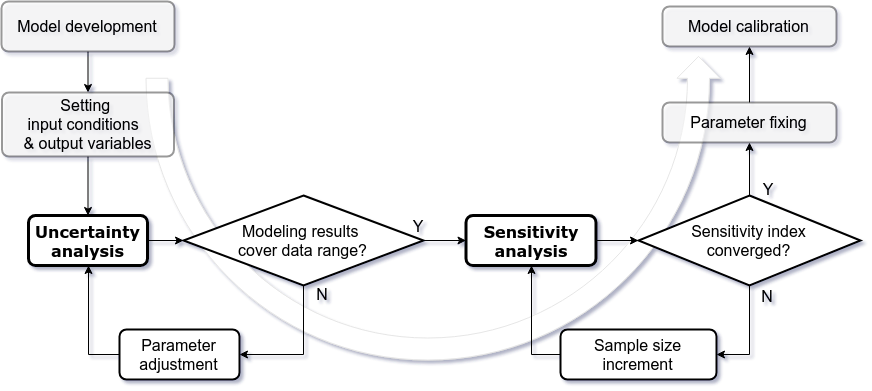
\includegraphics[width=1\linewidth]{workflow} 
\caption{The proposed workflow for performing uncertainty and sensitivity analysis in Bayesian MCMC model calibration process.}
\label{fig:workflow}
\end{figure}

\clearpage
\newpage

\begin{figure}
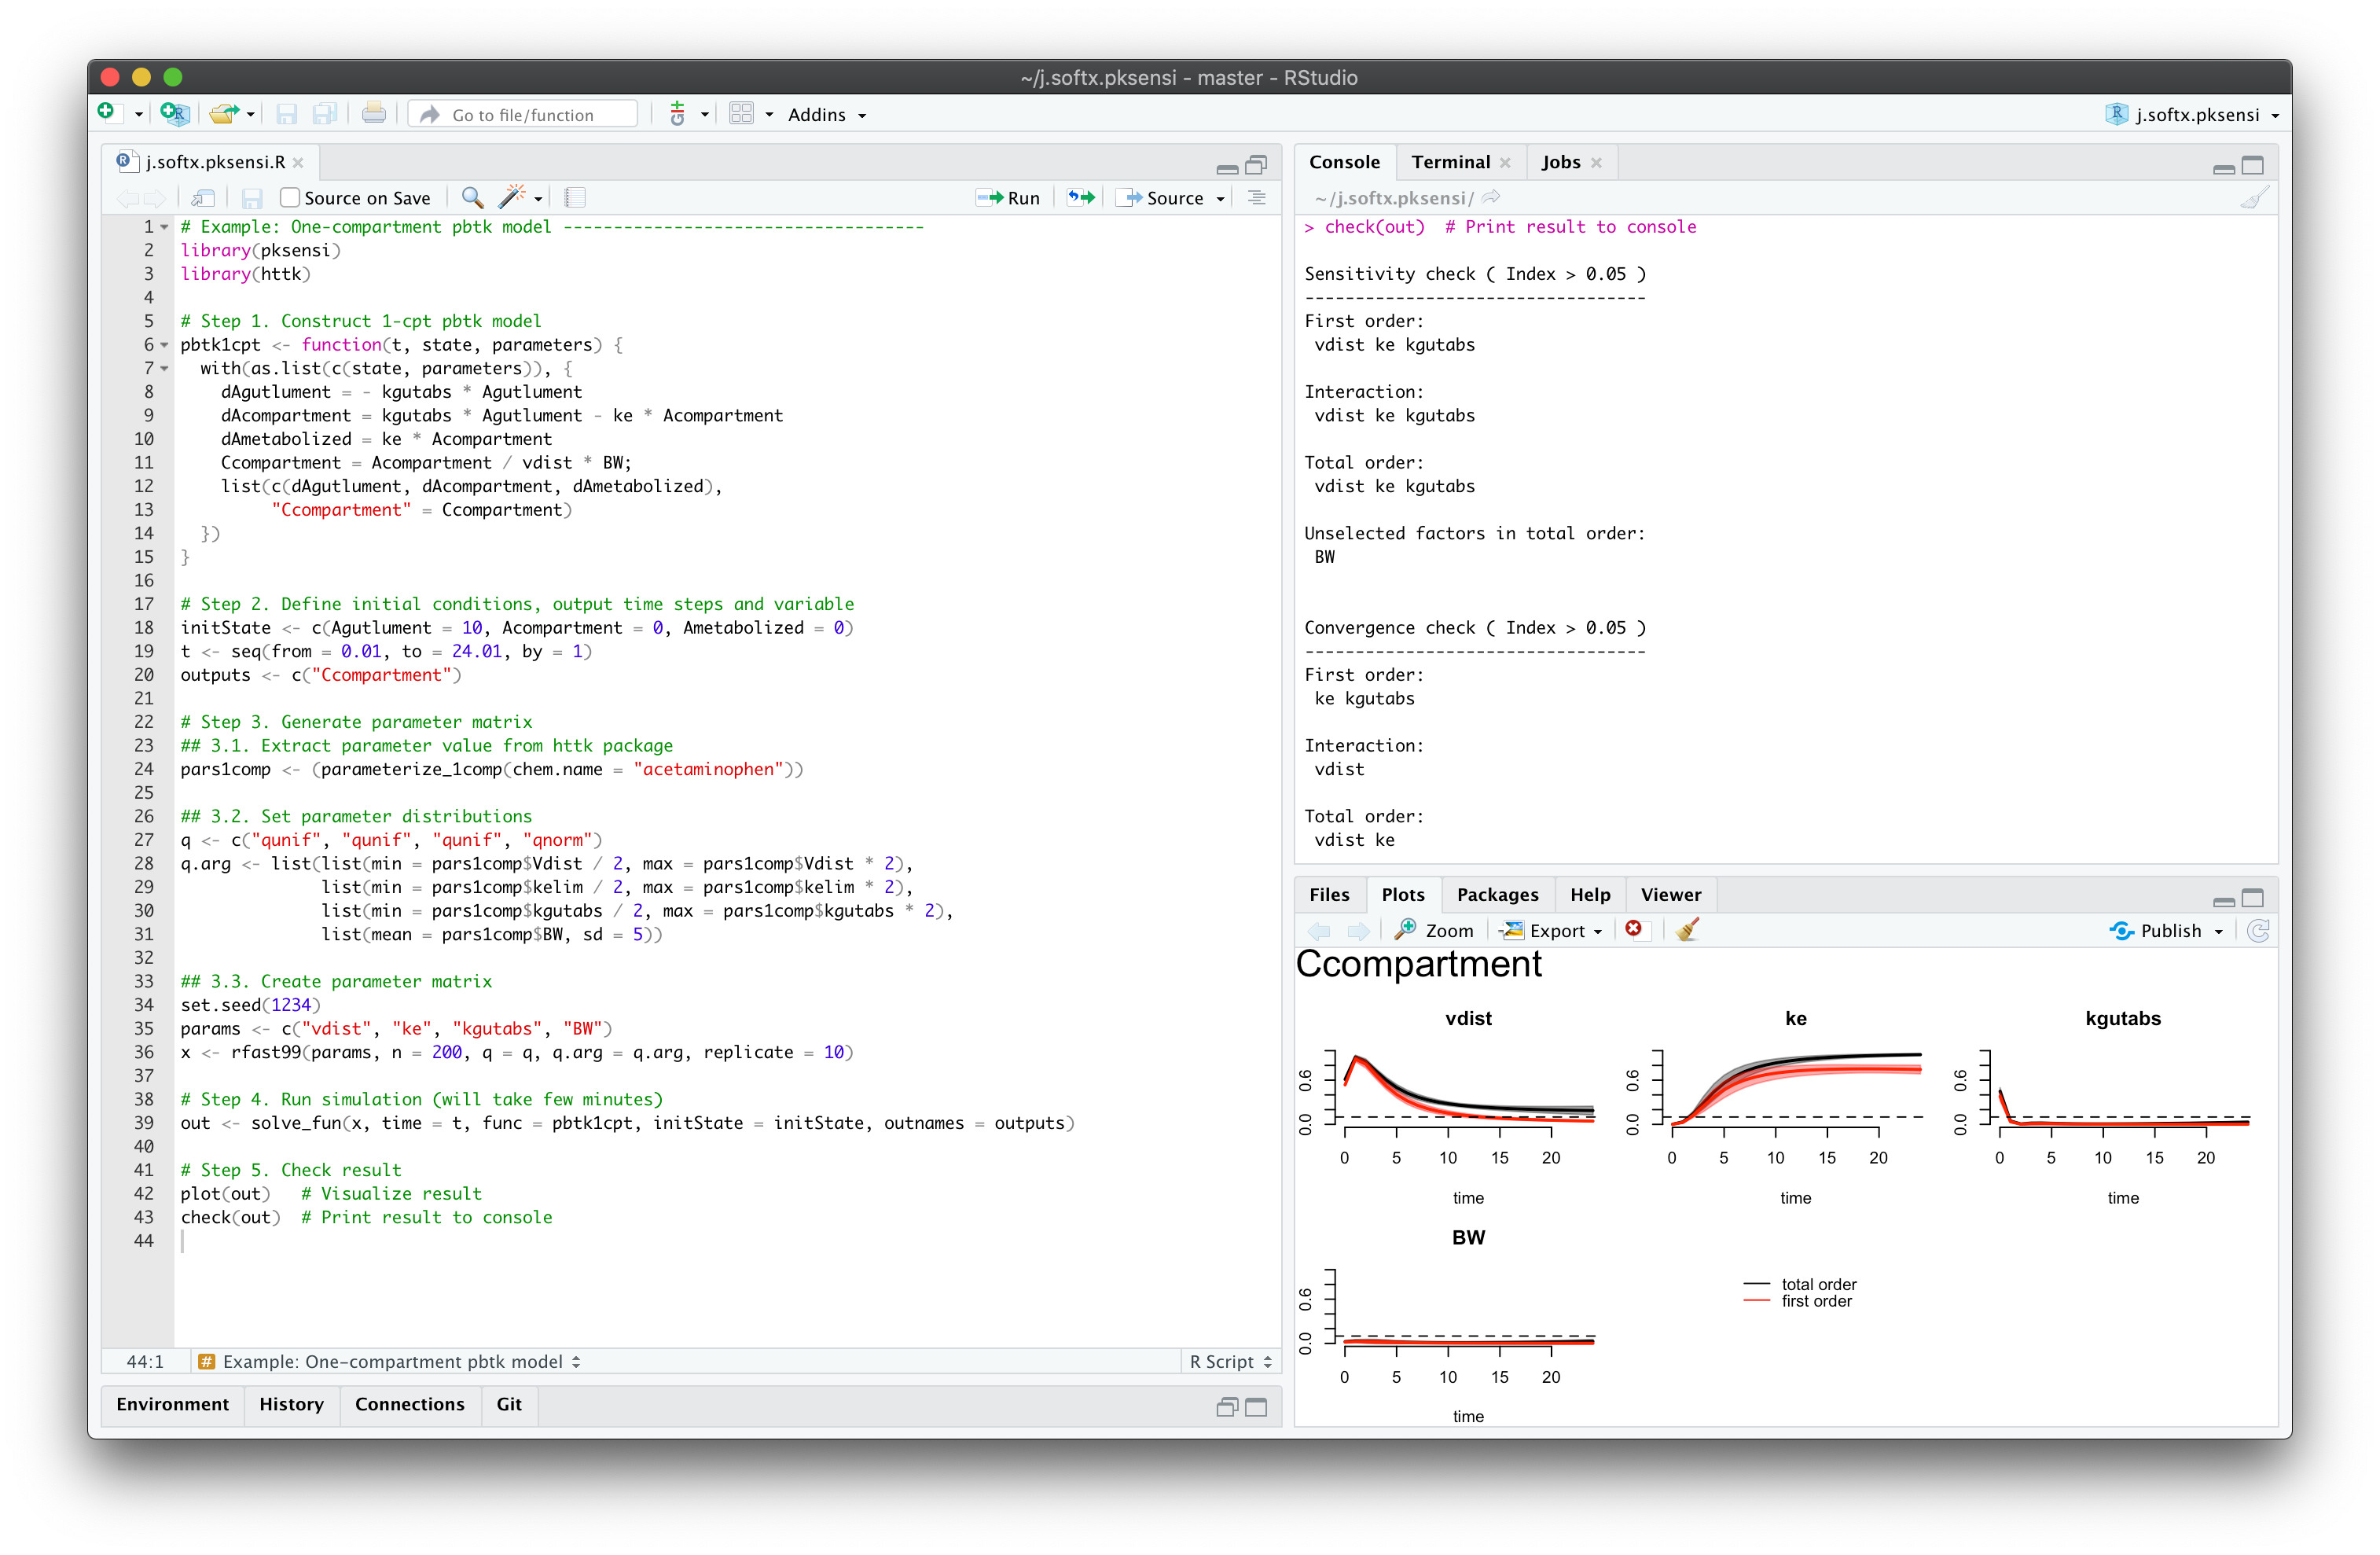
\includegraphics[width=1\linewidth]{example-1} 
\caption{Example R script and its corresponding results for the application of the \textbf{pksensi} in one-compartment pharmacokinetic modeling. The checking result can directly show in the R console through \textit{\textbf{check()}} function, and the visualization result can output by \textit{\textbf{plot()}} function.}
\label{fig:example-1}
\end{figure}

\clearpage
\newpage

\begin{figure}
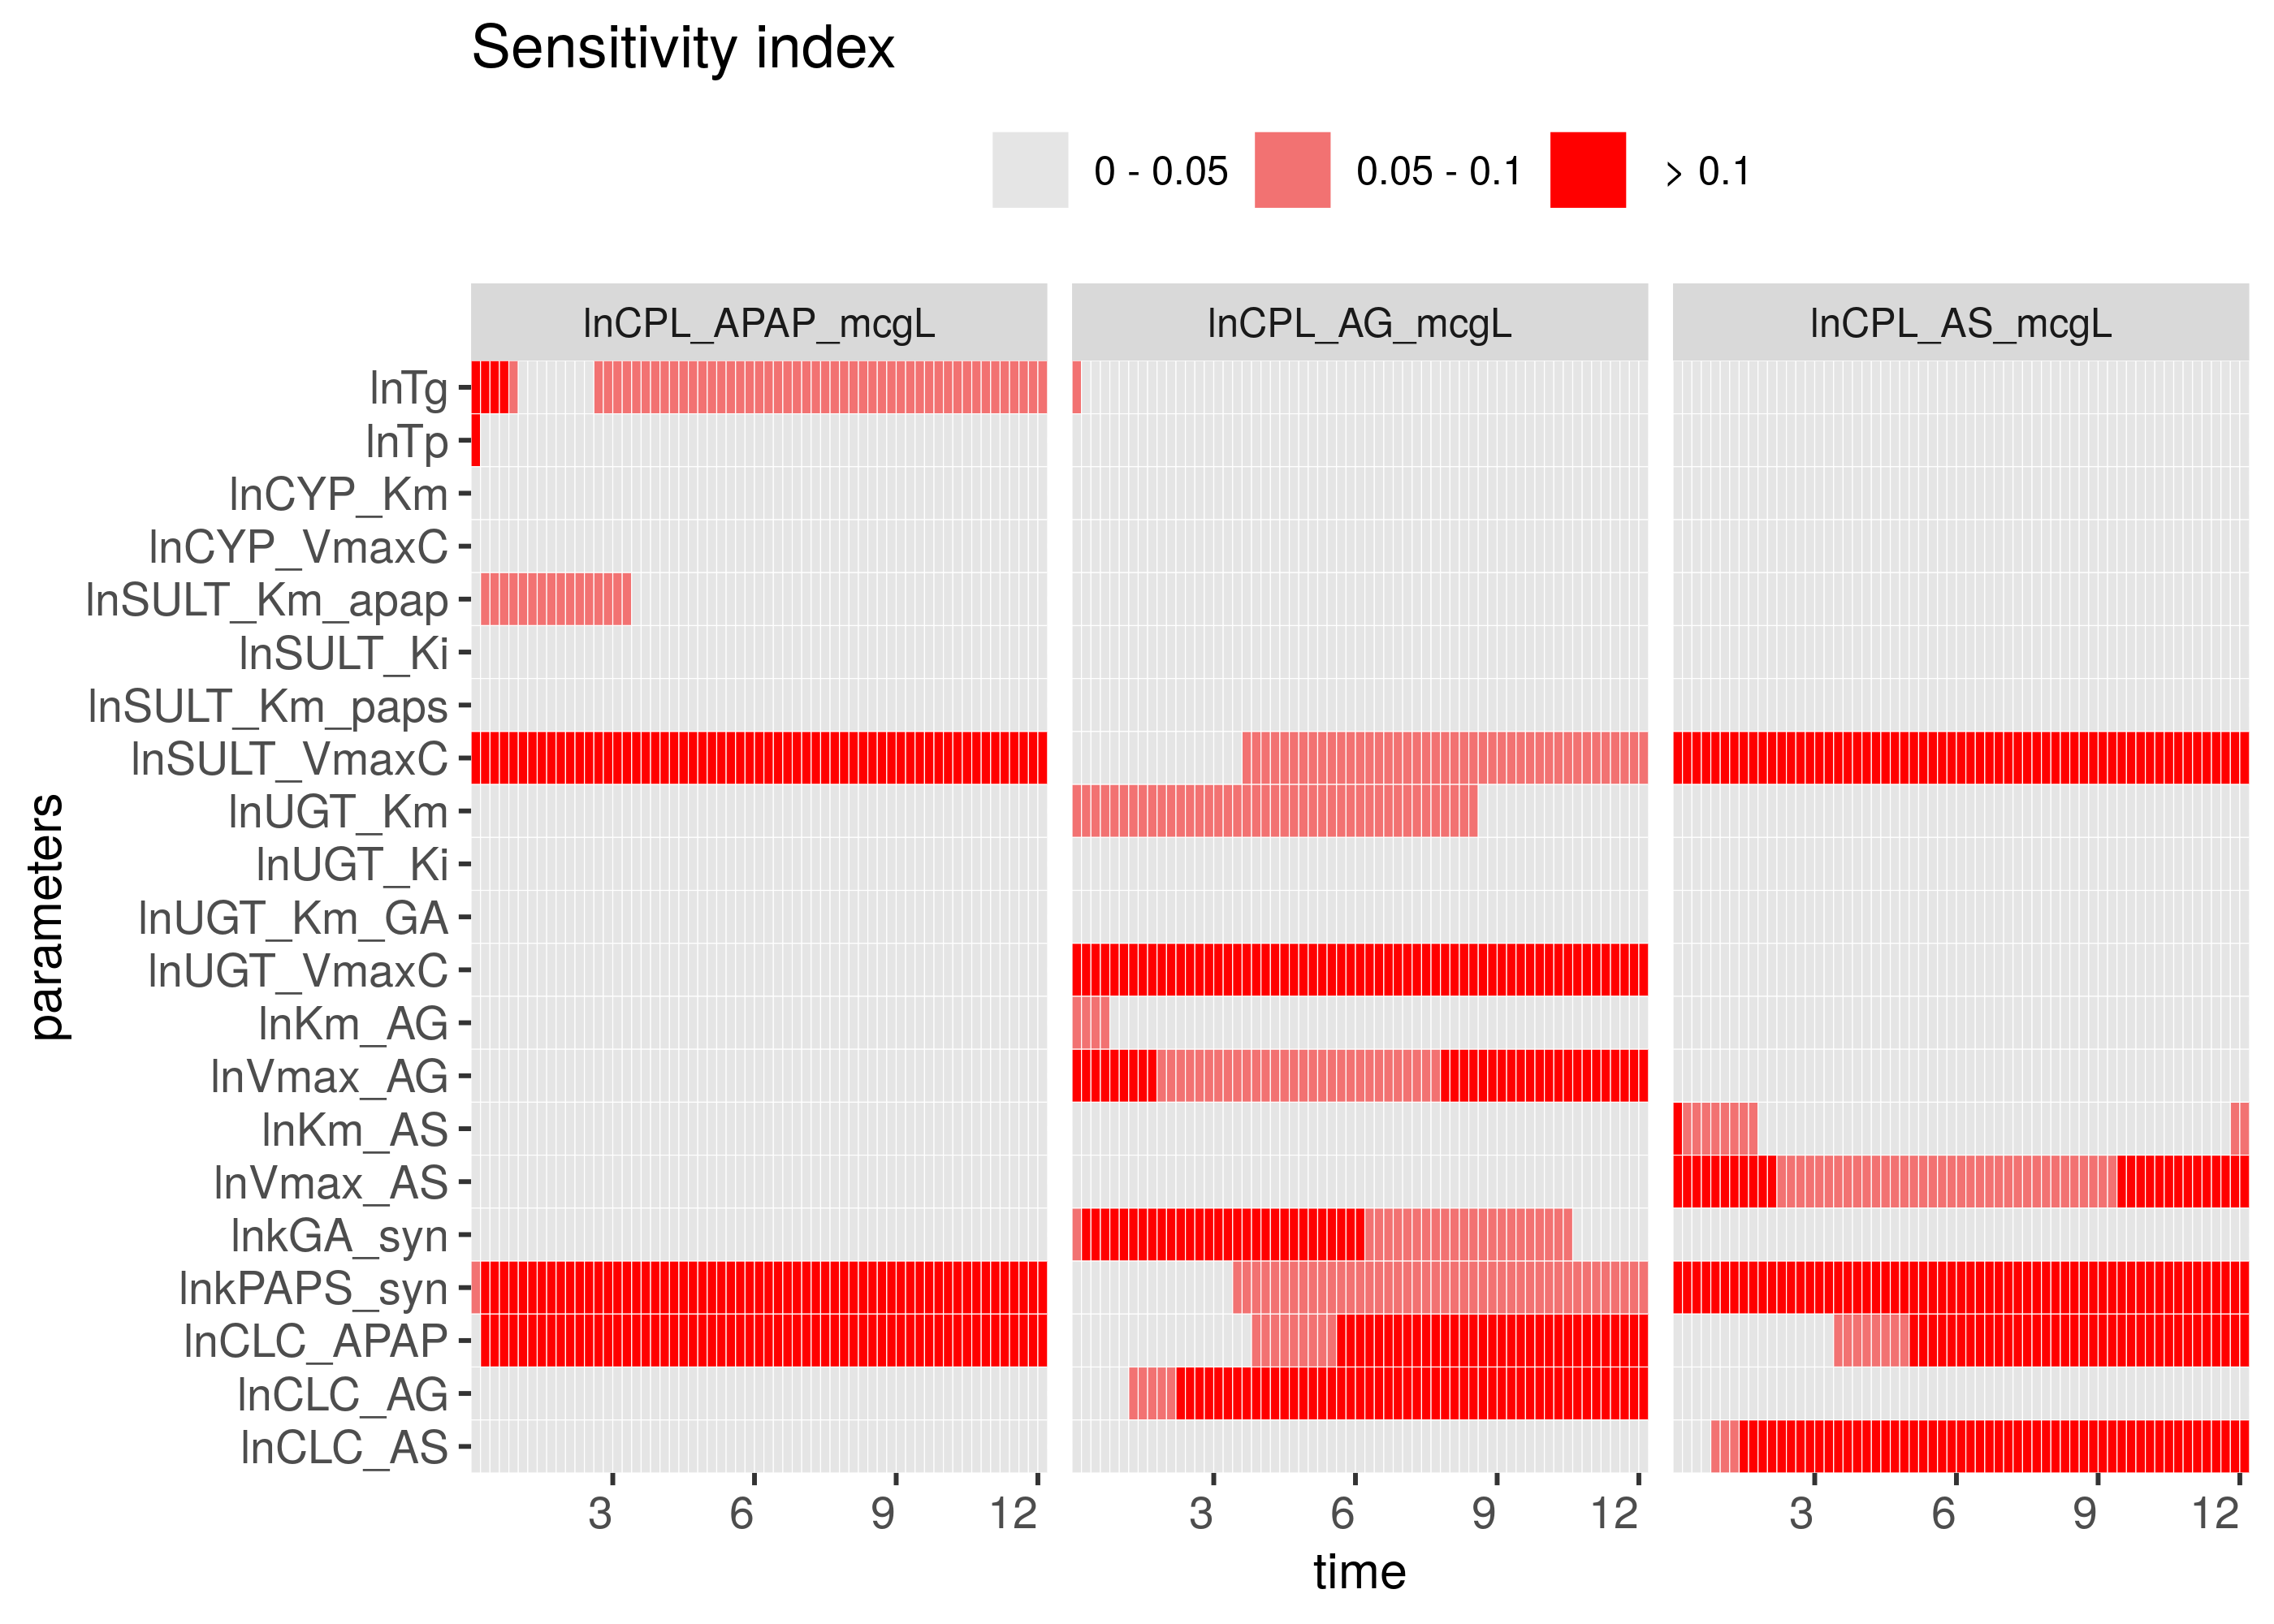
\includegraphics[width=1\linewidth]{example-2} 
\caption{Heat map representation of time-dependent total SI computed from 21 substance-specific parameters in APAP-PBPK model.}
\label{fig:example-2}
\end{figure}

\end{landscape}


\section*{Current executable software version}
\label{}

\begin{table}[!h]
\begin{tabular}{|l|p{6.5cm}|p{6.5cm}|}
\hline
\textbf{Nr.} & \textbf{(Executable) software metadata description} & \textbf{Please fill in this column} \\
\hline
S1 & Current software version & 1.2.0 \\
\hline
S2 & Permanent link to executables of this version  & \url{https://cran.r-project.org/web/packages/pksensi} \\
\hline
S3 & Legal Software License & GPL-3 \\
\hline
S4 & Computing platforms/Operating Systems & Linux, MacOS, Microsoft Windows \\
\hline
S5 & Installation requirements \& dependencies & ggplot2, data.table, deSolve, dplyr, getPass, magrittr, foreach, parallel, doParallel, reshape \\
\hline
S6 & If available, link to user manual - if formally published include a reference to the publication in the reference list & \url{https://cran.r-project.org/web/packages/pksensi/pksensi.pdf} \\
\hline
S7 & Support email for questions & \url{d99622005@ntu.edu.tw}\\
\hline
\end{tabular}
\caption{Software metadata (optional)}
\label{} 
\end{table}

\end{document}

%%
%% End of file `SoftwareX_article_template.tex'.
